\documentclass[]{beamer}
\usepackage{graphicx} 
\graphicspath{{Images/}{./}}
\usepackage{booktabs}
\usepackage{tikz}
\usepackage{pgfplots}
\usepackage{float}
\usepackage{listings,xcolor}

\usetheme{Madrid}
\usecolortheme{beaver}
\usefonttheme{default} 
\usepackage{palatino}
\usepackage[default]{opensans}
\useinnertheme{default}
\usepackage[german]{babel}
\usepackage{caption}



\setbeamertemplate{footline}{}
\setbeamertemplate{navigation symbols}{}
\setbeamertemplate{headline}{}


\title[]{Endpräsentation}

\author[shortname]{David Metzler \and Emircan Tutar  \and Niklas Kleiser}

\institute[shortinst]{ Hochschule Ravensburg Weingraten\\ \smallskip} 

\date{ \today}
%----------------------------------------------------------------------------------------

\begin{document}


%----------------------------------------------------------------------------------------
%	TITLE SLIDE
%----------------------------------------------------------------------------------------

\begin{frame}
	\titlepage % Output the title slide, automatically created using the text entered in the PRESENTATION INFORMATION block above
\end{frame}

%----------------------------------------------------------------------------------------
%	TABLE OF CONTENTS SLIDE
%----------------------------------------------------------------------------------------

% The table of contents outputs the sections and subsections that appear in your presentation, specified with the standard \section and \subsection commands. You may either display all sections and subsections on one slide with \tableofcontents, or display each section at a time on subsequent slides with \tableofcontents[pausesections]. The latter is useful if you want to step through each section and mention what you will discuss.

%\begin{frame}
	%\frametitle{Presentation Overview} % Slide title, remove this command for no title

	%\tableofcontents % Output the table of contents (all sections on one slide)
	%\tableofcontents[pausesections] % Output the table of contents (break sections up across separate slides)
%\end{frame}

%----------------------------------------------------------------------------------------
%	PRESENTATION BODY SLIDES
%----------------------------------------------------------------------------------------

\section{Systemaufbau}
\begin{frame}{Systemaufbau}

	\begin{figure}
		\begin{tikzpicture}[scale=0.76]

			\draw [-, dashed, gray] (4,1)-- (-4,1)--(-4,3.5) --(4,3.5) --(4,1);
			\node at (-2.8 ,3) {BED VIEW};

			\node[inner sep=0pt] (whitehead) at (2,2.5)
			{
\includegraphics[width=.05\textwidth]{Images/camera.png}};

			\node[above] at (2.2,2.6) {\scriptsize Raspberry Pi};

			\node[inner sep=0pt] (whitehead) at (0,2)
			{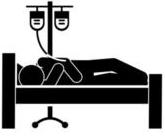
\includegraphics[width=.1\textwidth]{Images/person_in_bed.png}};

			\node at (-2.5 ,-1) {ROOM VIEW};

			\draw [-, dashed, gray] (4,-0.5)-- (-4,-0.5)--(-4,-4) --(4, -4 ) --(4,-0.5);

			\node[inner sep=0pt] (whitehead) at (2,-1.5)
			{
\includegraphics[width=.05\textwidth]{Images/camera.png}};



			\node[inner sep=0pt] (whitehead) at (-0.25,-1.25)
			{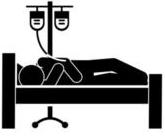
\includegraphics[width=.1\textwidth]{Images/person_in_bed.png}};


			\node[inner sep=0pt] (whitehead) at (0,-2.25)
			{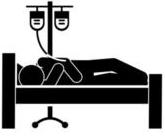
\includegraphics[width=.1\textwidth]{Images/person_in_bed.png}};

			\node[inner sep=0pt] (whitehead) at (-0.5,-3.25)
			{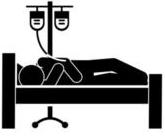
\includegraphics[width=.1\textwidth]{Images/person_in_bed.png}};


			\node[inner sep=0pt] (whitehead) at (4.0,0.25)
			{
\includegraphics[width=.06\textwidth]{Images/server.png}};

			\node[below] at (2.2,-1.6) {\scriptsize Raspberry Pi};

			\node[below] at (4.0,0) {\scriptsize Broker};



			\draw [-] (2,2.5)-- ( 3,2.5) -- (3,0.25) ;
			\draw [-] (2,-1.5)-- ( 3,-1.5) -- (3,0.25) ;
			\draw [-]  (3,0.25)  -- (3.8,0.25);

			\draw [->]  (4.2 ,0.25) -- (5.0,0.25) -- (5.0,-1.5) -- (5.5,-1.5);
			\draw [->]  (4.2 ,0.25) -- (5.0,0.25) -- (5.0,2.5) -- (5.5,2.5);

			\node at  (7.0,2.5) {\scriptsize Bed Detection};


			\node at  (7.0,-1.5) {\scriptsize Fall Detection};



			\draw [->]  (8.5 ,-1.5) -- (9.0,-1.5) -- (9,0.25) -- (9.5,0.25)  ;

			\draw [->]  (8.5, 2.5) -- (9.0,2.5) -- (9,0.25) -- (9.5,0.25) ;

			\node[inner sep=0pt] (whitehead) at (9.85,0.25)
			{
\includegraphics[width=.05\textwidth]{Images/raspi.png}};

			\node[below] at (9.8,-0.1) {\scriptsize Pi };

			\draw [->]  (10.3,0.25) -- (10.6,0.25) ;

			\node[red] at  (11.4,0.25) {Alarm};


		\end{tikzpicture}
		\caption{Darstellung des Systemaufbaus}
		\label{fig:patient_monitoring}

	\end{figure}


\end{frame}

\section{Lastenheft}
\subsection{Muss - Anforderungen}
\begin{frame}
	\frametitle{Lastenheft}
	\framesubtitle{Muss - Anforderungen}
	\begin{enumerate}
		\item Docker \checkmark 
		\item Ubuntu 22.04 (LTS) \checkmark  
		\item Dynamisches DNS-Management (ddclient) \checkmark 
		\item Fail2ban \checkmark 
		\item MQTT / MQTT-Client \checkmark 
		\item SMTP-Server / SMTP-Client \checkmark 
		\item Raspberry und Raspberry Pi  \checkmark 
		\item Fall Detektion \checkmark 
		\item Matrix \checkmark 
	\end{enumerate}
\end{frame}

\subsection{Soll - Anforderungen}
\begin{frame}
	\frametitle{Lastenheft}
	\framesubtitle{Soll - Anforderungen}
	\begin{enumerate}
		\item Bett Detektion
		\item Alarm (Ton und Licht) \checkmark 
		\item Firewall \checkmark  
	\end{enumerate}
\end{frame}

\subsection{Kann - Anforderungen}
\begin{frame}
	\frametitle{Lastenheft}
	\framesubtitle{Kann - Anforderungen}
	\begin{enumerate}
		\item MQTT Frontend
		\item Gesprochene Information über Patient in Hilfesituation
		\item Kameraview \checkmark 
	\end{enumerate}
\end{frame}



\section{Aktueller Stand}
\subsection{Setup Hardware}
\begin{frame}
	\frametitle{Setup}
	\framesubtitle{Hardware}
	\begin{enumerate}
		\item 2  Raspberry Pi und 1 Atomic Pi
		\item 1 Kamera ist da
		\item Ubuntu 22.04 installiert
	\end{enumerate}
\end{frame}


\section{Aktueller Stand}
\subsection{Raspberry PI}
\begin{frame}
	\frametitle{Setup}
	\framesubtitle{Raspberry PI}
	\begin{figure}
		\centering
		\begin{minipage}[t]{0.45\textwidth}
			\centering
			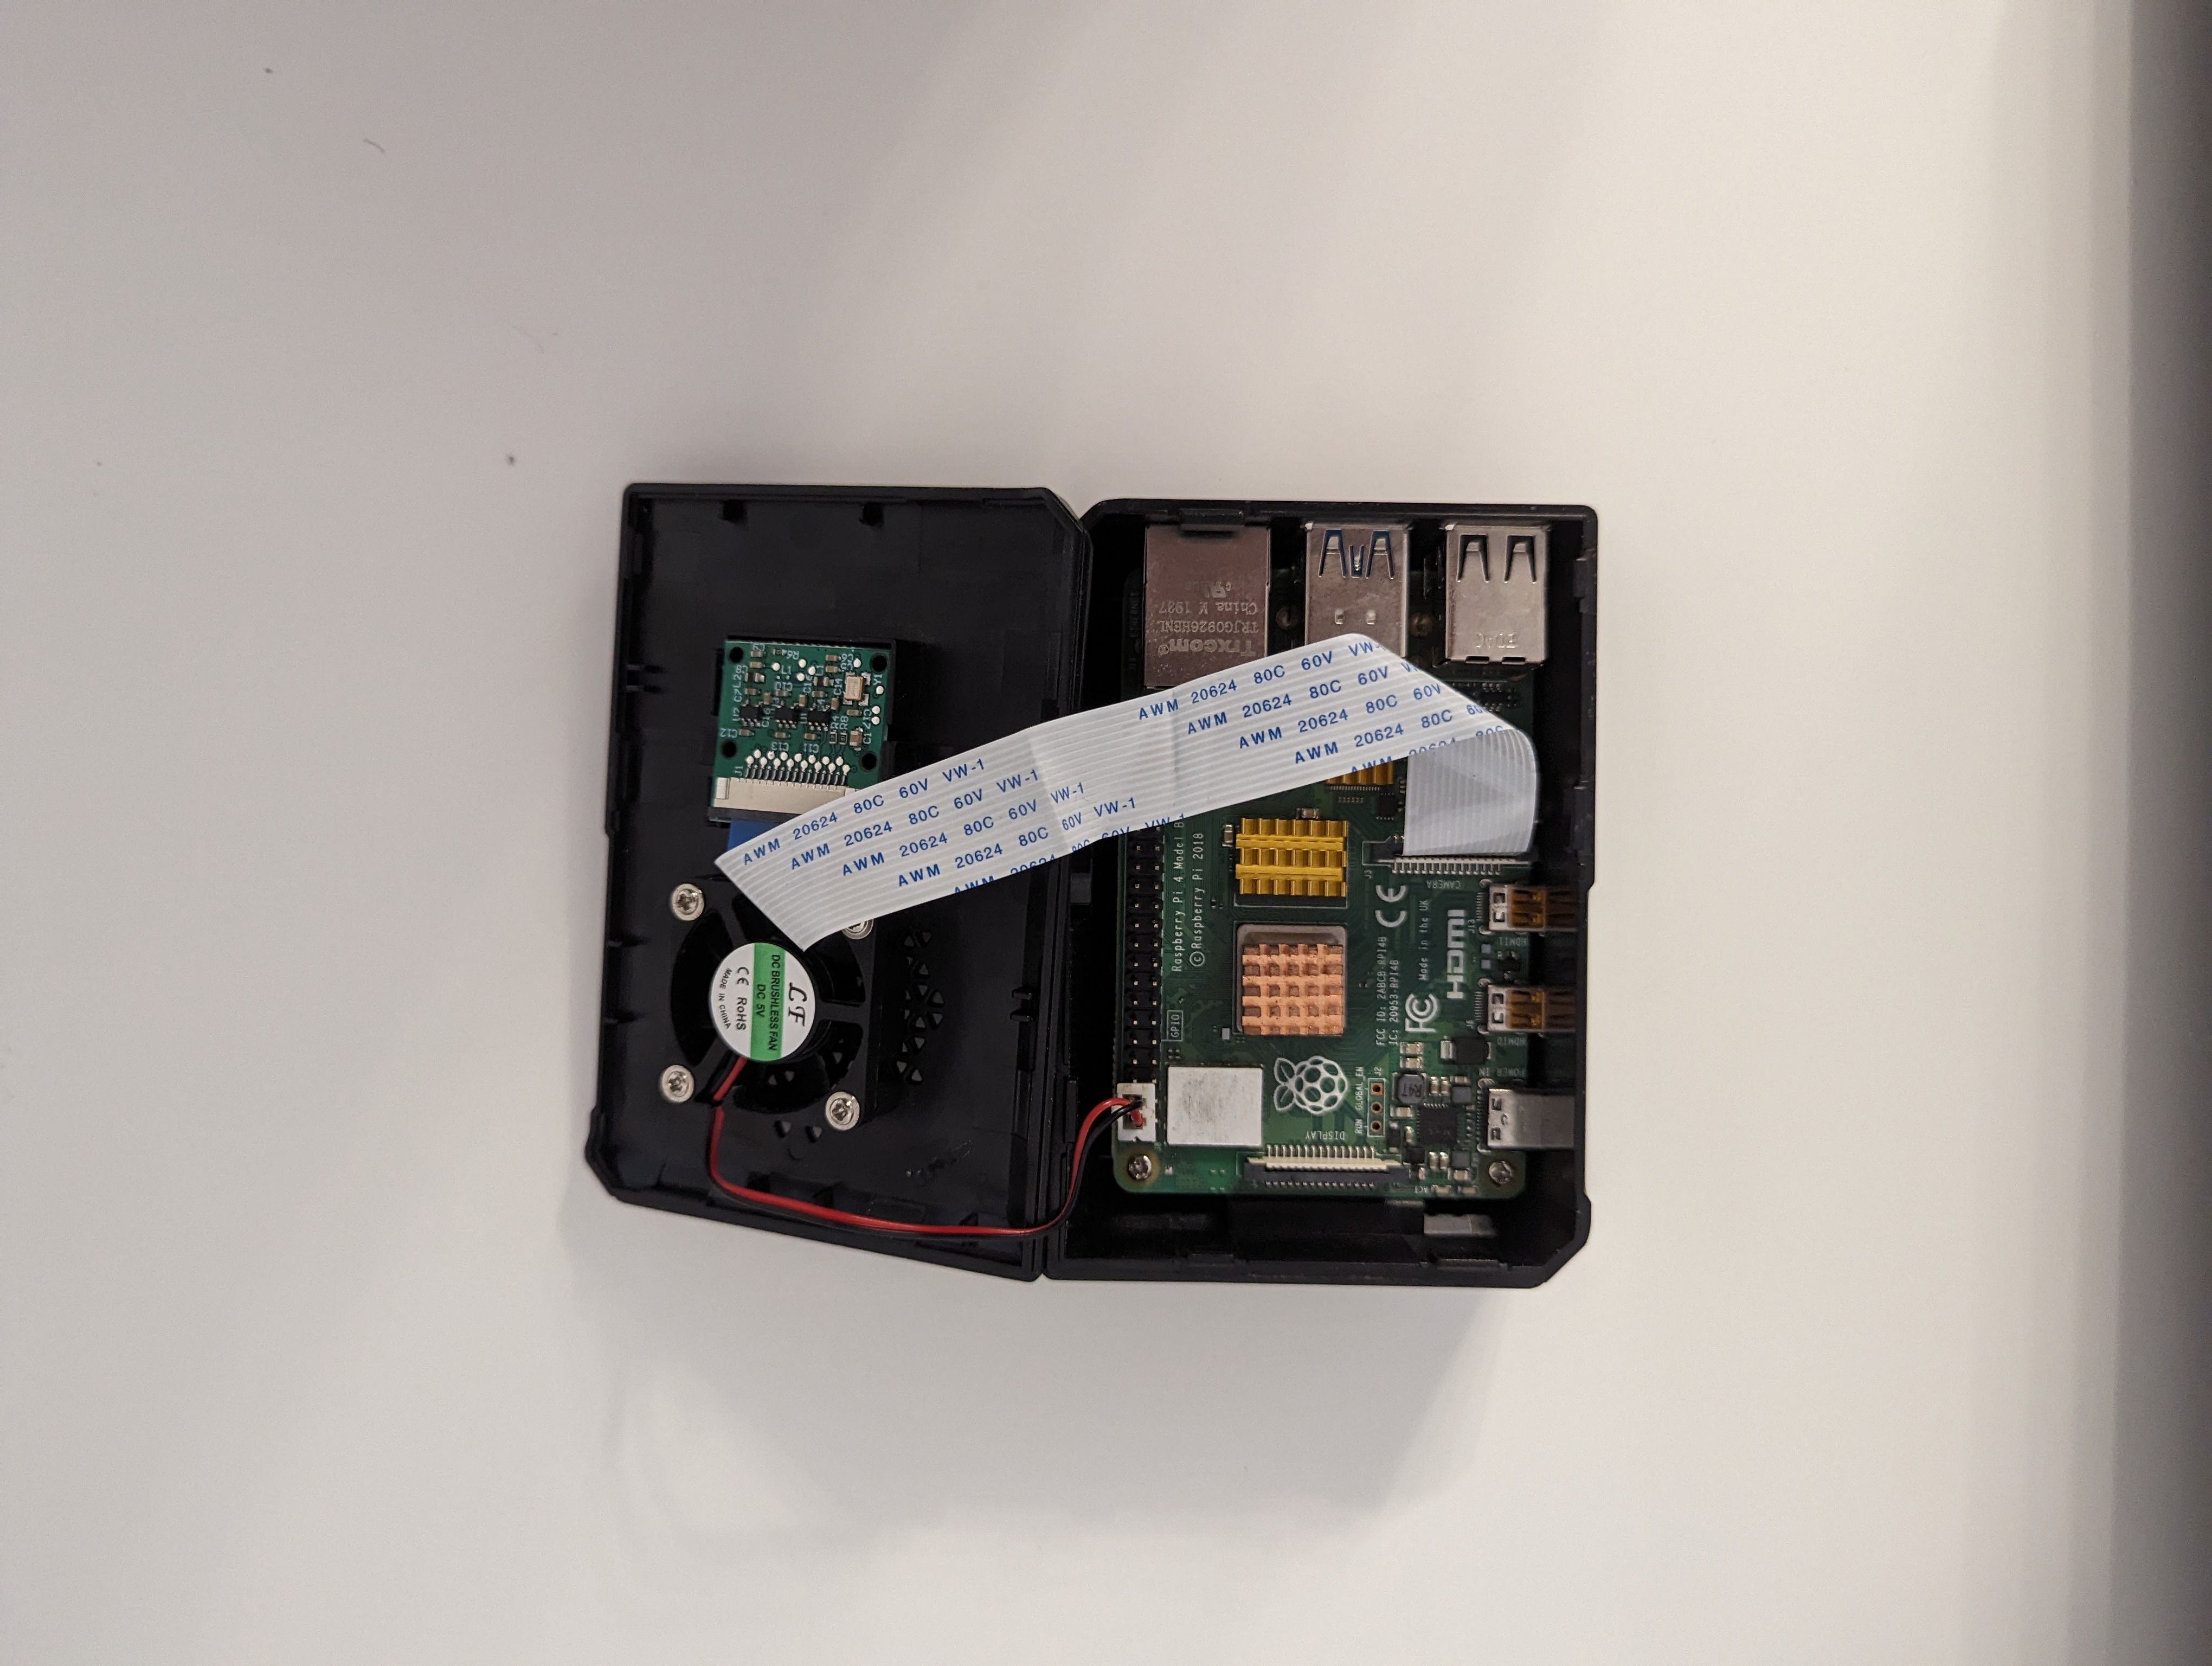
\includegraphics[width=0.8\textwidth]{Images/Raspberry_Pi_and_Camera_Open.jpg}
			\caption*{Aufbau im Gehäuse}
		\end{minipage}
		\hfill
		\begin{minipage}[t]{0.45\textwidth}
			\centering
			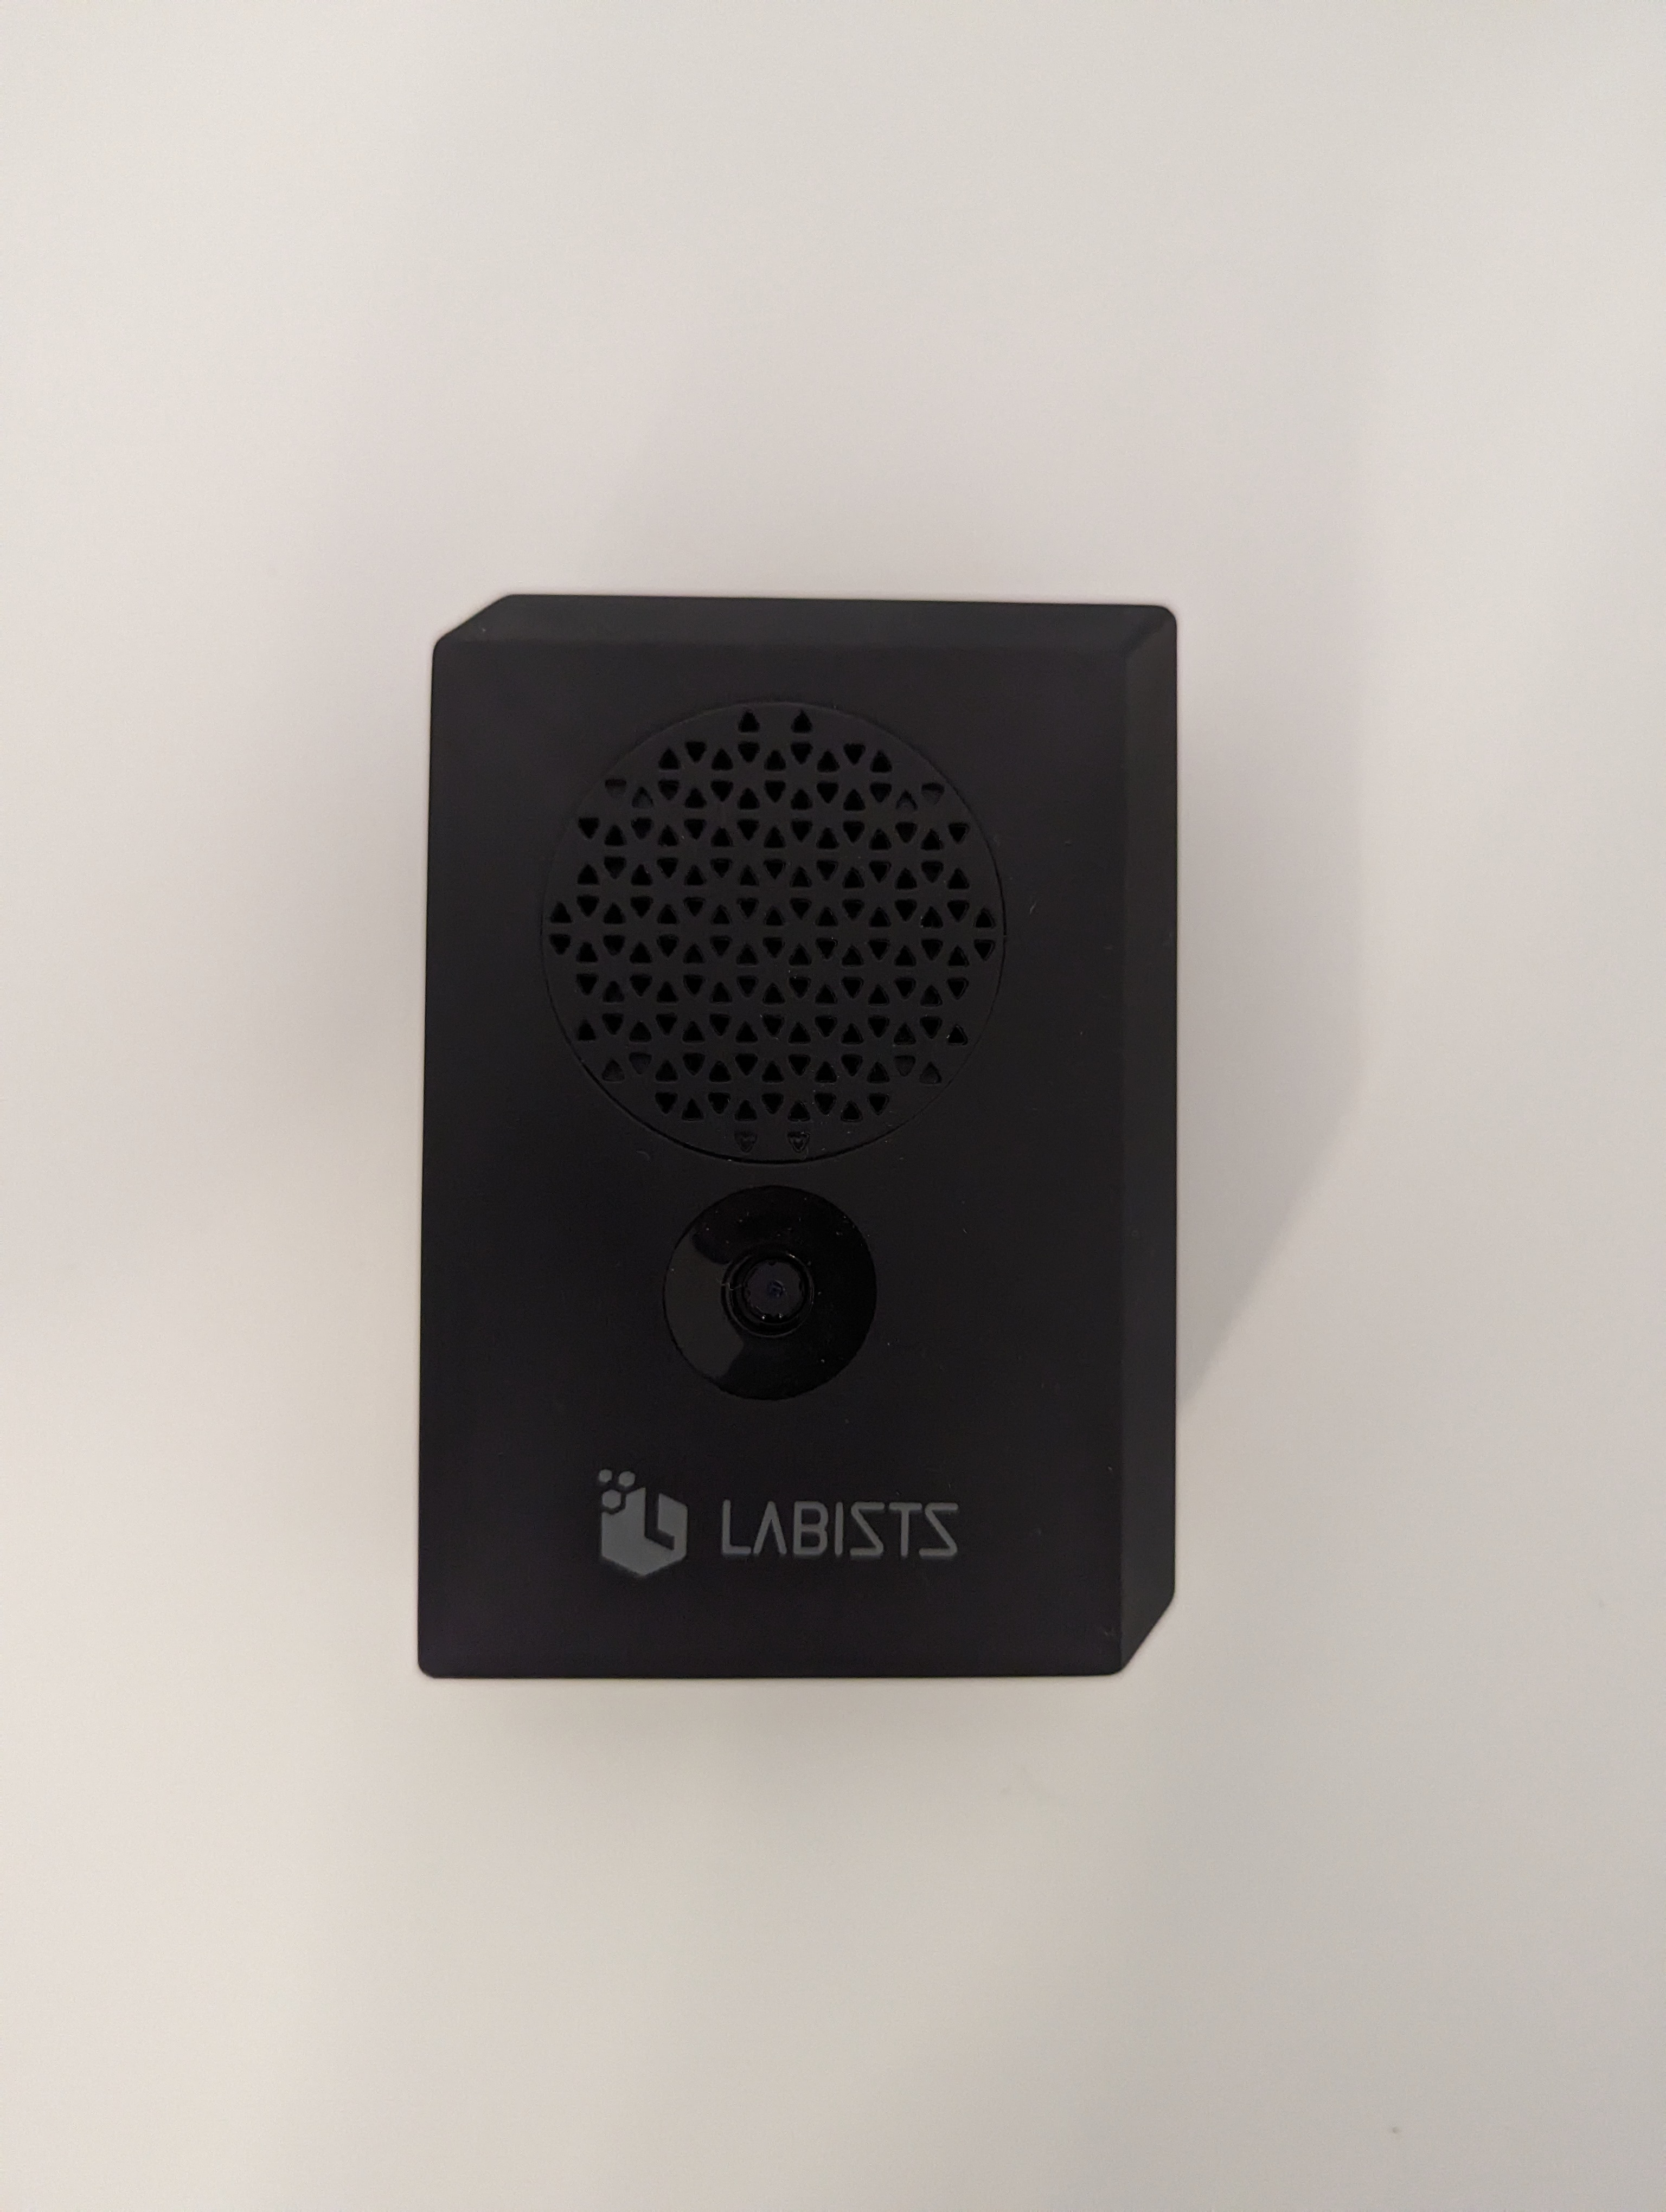
\includegraphics[width=0.6\textwidth]{Images/Raspberry_Pi_and_Camera_Closed.jpg}
			\caption*{Gehäuse mit Kamera}
		\end{minipage}
		\hfill
		\caption{Raspberry Pi mit Kamera}
		\label{fig:Raspberry PI}
	\end{figure}
\end{frame}

\subsection{Atomic PI}
\begin{frame}
	\frametitle{Setup}
	\framesubtitle{Atomic PI}
	\begin{figure}
		\centering
		\begin{minipage}[t]{1\textwidth}
			\centering
			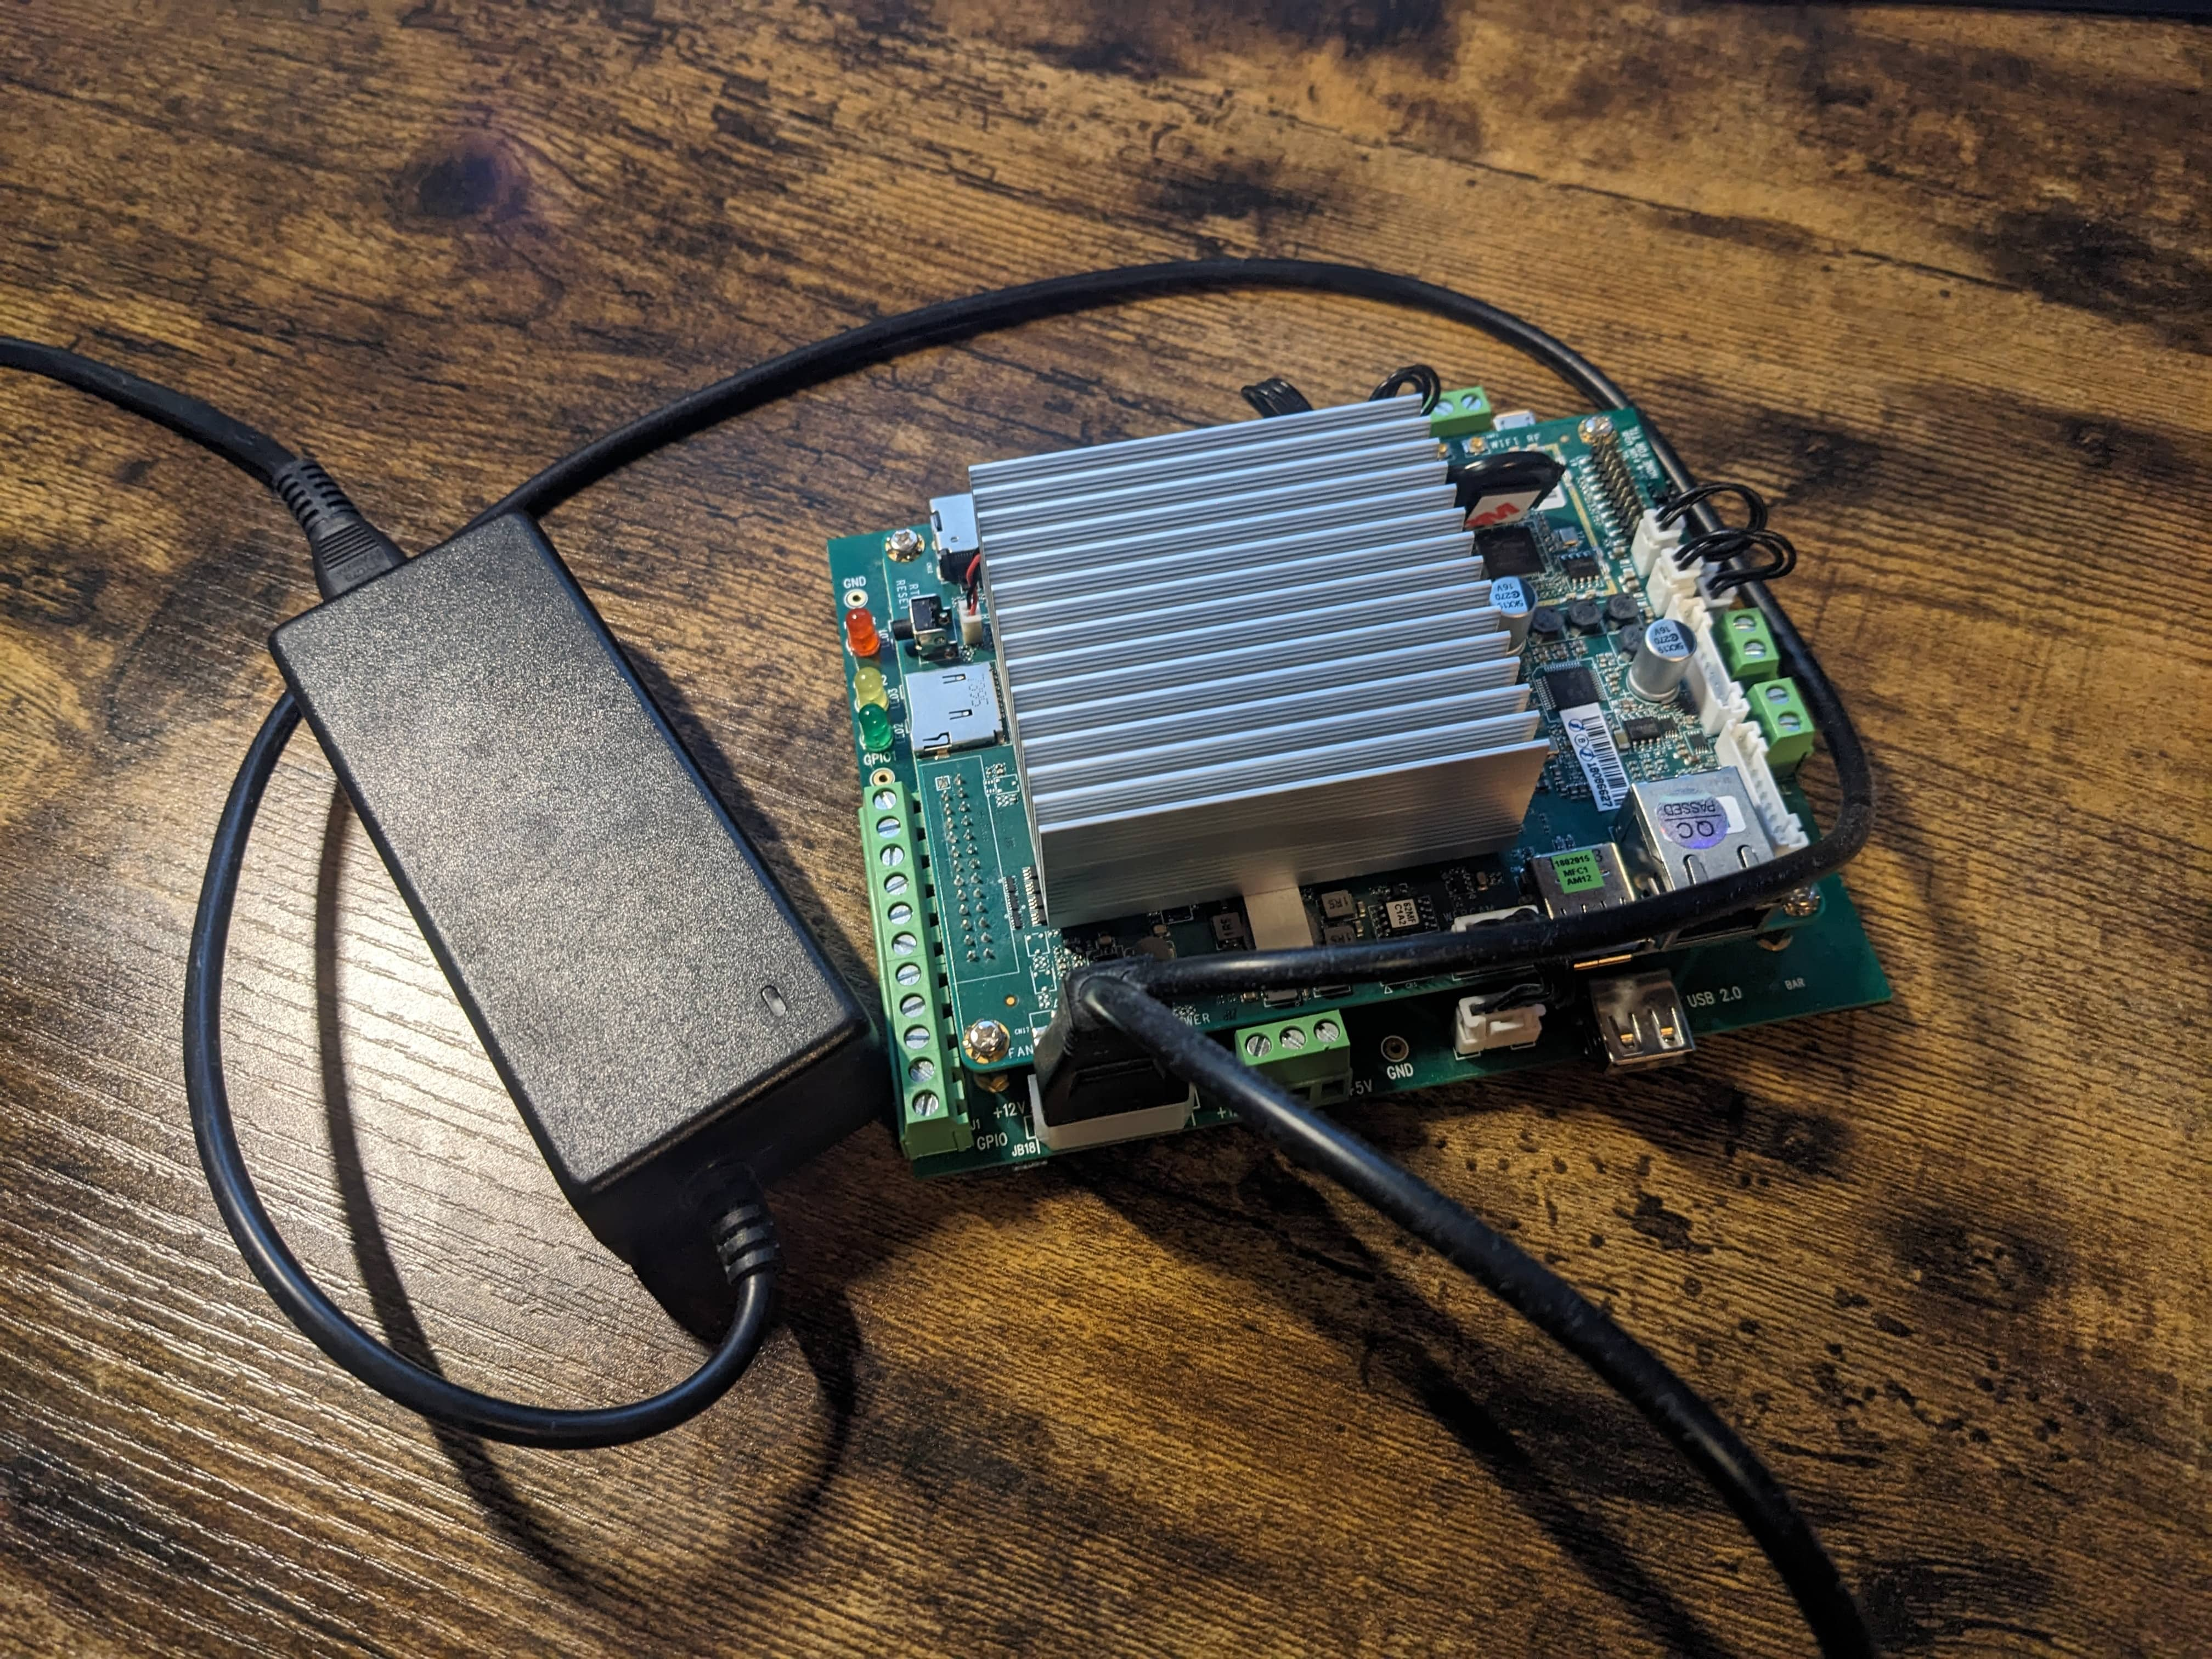
\includegraphics[width=0.8\textwidth]{Images/AtomicPi.jpg}
		\end{minipage}
		\caption{Atomic Pi}
		\label{fig:Atomic Pi}
	\end{figure}
\end{frame}




\subsection{Alarm}

\begin{frame}
	\frametitle{Aktueller Stand}
	\framesubtitle{Alarm-Setup}
	\begin{figure}
		\centering
		\begin{minipage}{0.32\textwidth}
			\centering
			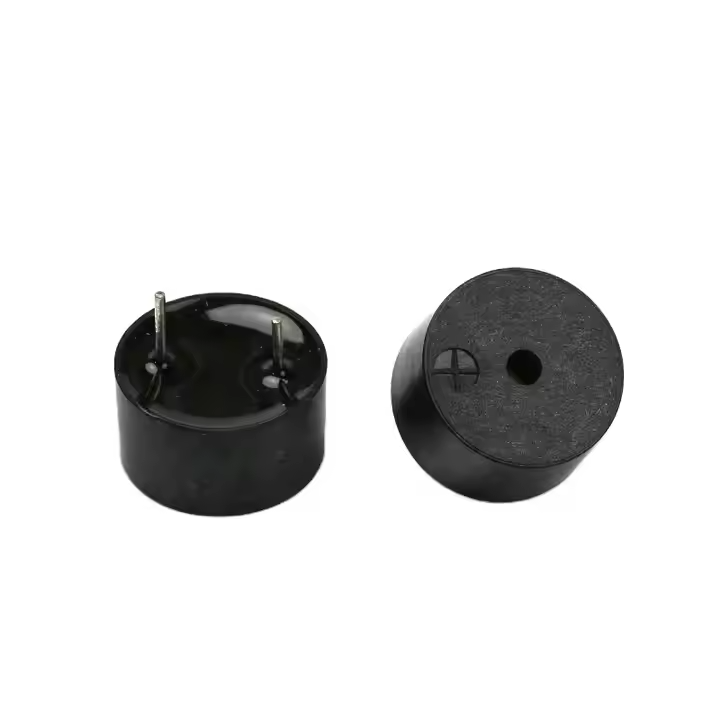
\includegraphics[width=\textwidth]{Images/HXD_Buzzer_Pipser.png} 
			\caption{HXD - als Alarm-Pipser}
		\end{minipage}\hfill
		\begin{minipage}{0.32\textwidth}
			\centering
			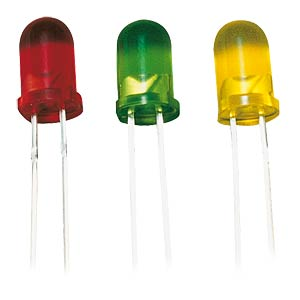
\includegraphics[width=\textwidth]{Images/Leds.png} 
			\caption{Leds}
		\end{minipage}\hfill
		\begin{minipage}{0.32\textwidth}
			\centering
			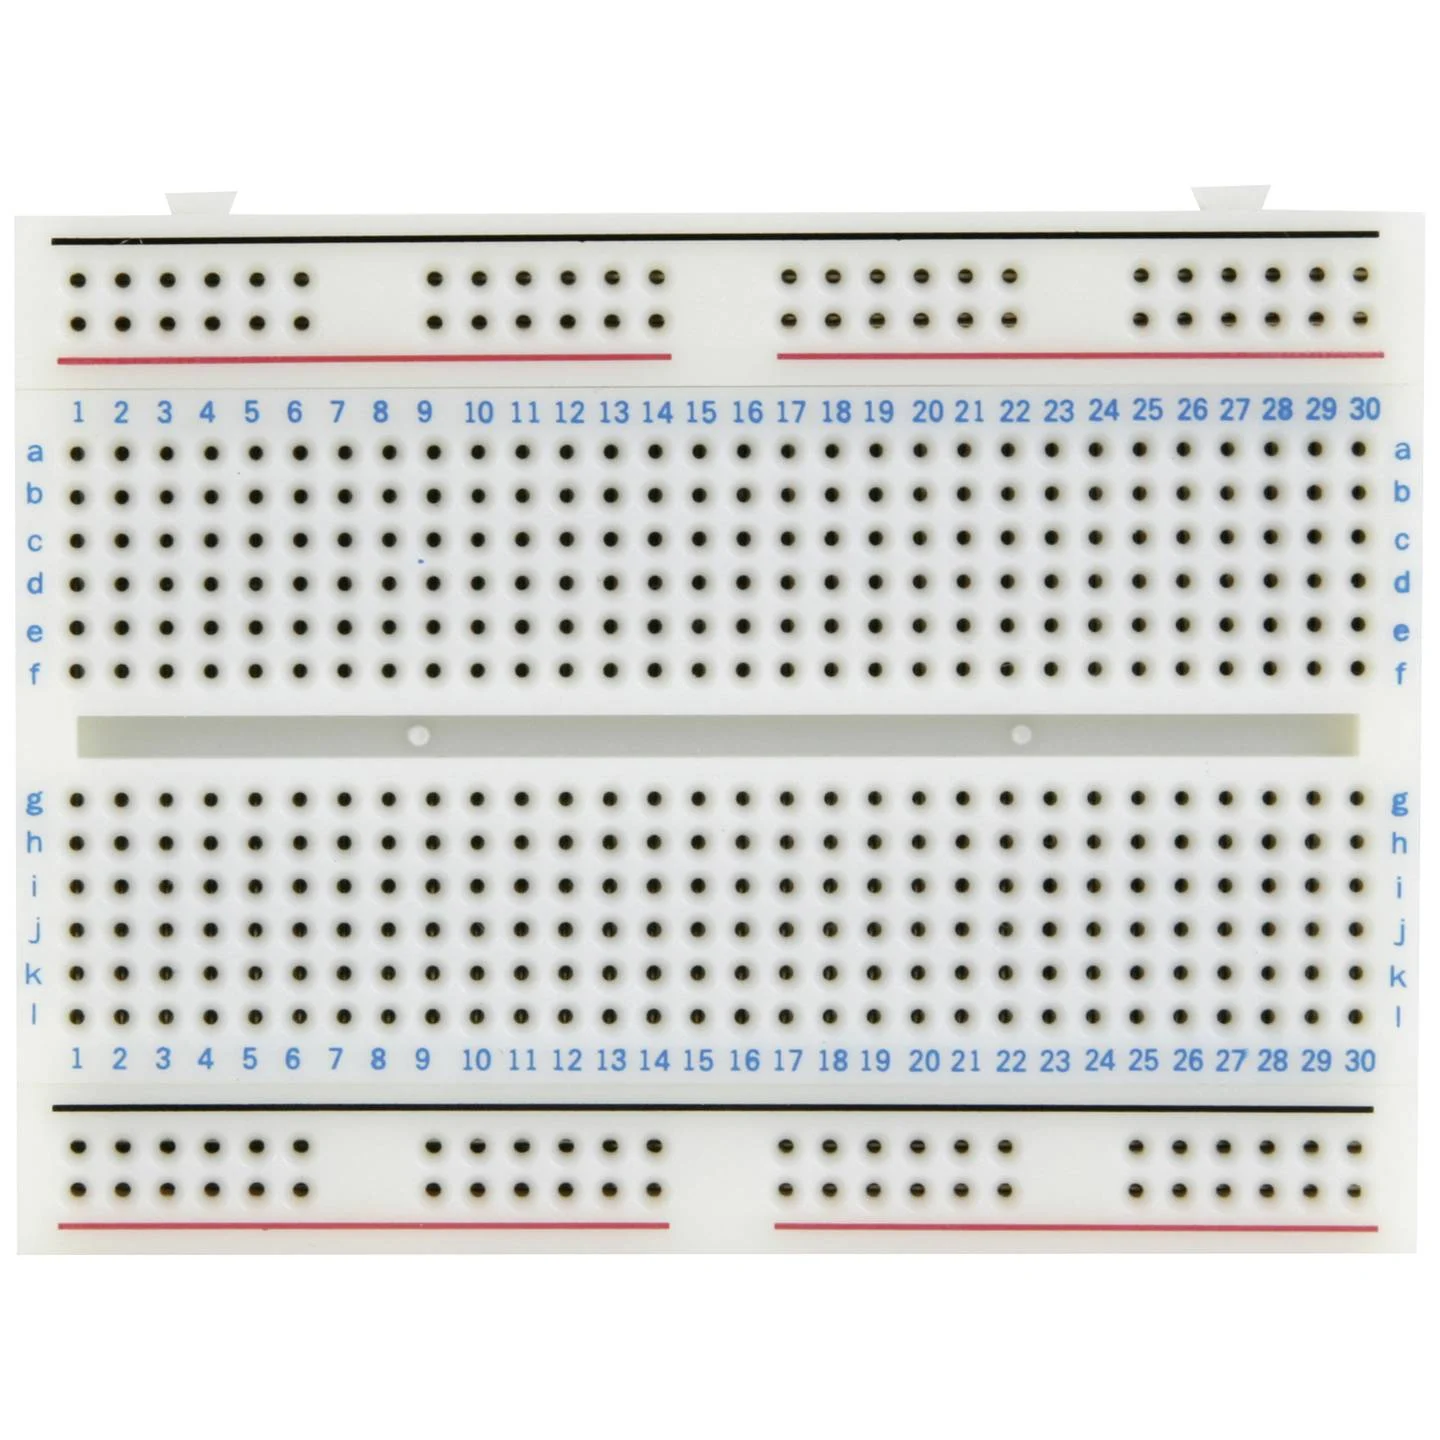
\includegraphics[width=\textwidth]{Images/Steckbrett.png}
			\caption{Steckboard}
		\end{minipage}
	\end{figure}
	
\end{frame}

\subsection{Video}

\begin{frame}
	\frametitle{Video}
	
\end{frame}


\subsection{Docker}
\begin{frame}
	\frametitle{Docker}
	
	\begin{enumerate}
		\item Docker 
		\item Docker Compose
		\item Environment Variablen
	\end{enumerate}
\end{frame}


\subsection{MQTT}
\begin{frame}
	\frametitle{MQTT}

	\begin{enumerate}
		\item Konzept ausgearbeitet
		\item Erste Implementation
		\item Erfolgreich auf AtomicPi deployt
		\item Test Publisher \& Subscriber haben funktioniert
	\end{enumerate}
\end{frame}

\subsection{SMTP-Server / SMTP-Client}
\begin{frame}
	\frametitle{Mailcow}
	\framesubtitle{SMTP-Server / SMTP-Client}
	\begin{enumerate}
		\item DNS - Setup erledigt
		\item Mailcow deployt
		\item SOGo Weboberfläche deployt
		\item Erfolgreich Testmails an eigenes Postfach geschickt
		\item Herausforderung: Disk Space
	\end{enumerate}
\end{frame}

\begin{frame}
	\frametitle{SOGo Weboberfläche}
	\framesubtitle{SMTP-Server / SMTP-Client}
	\begin{figure}
		\begin{minipage}[t]{1\textwidth}
			\centering
			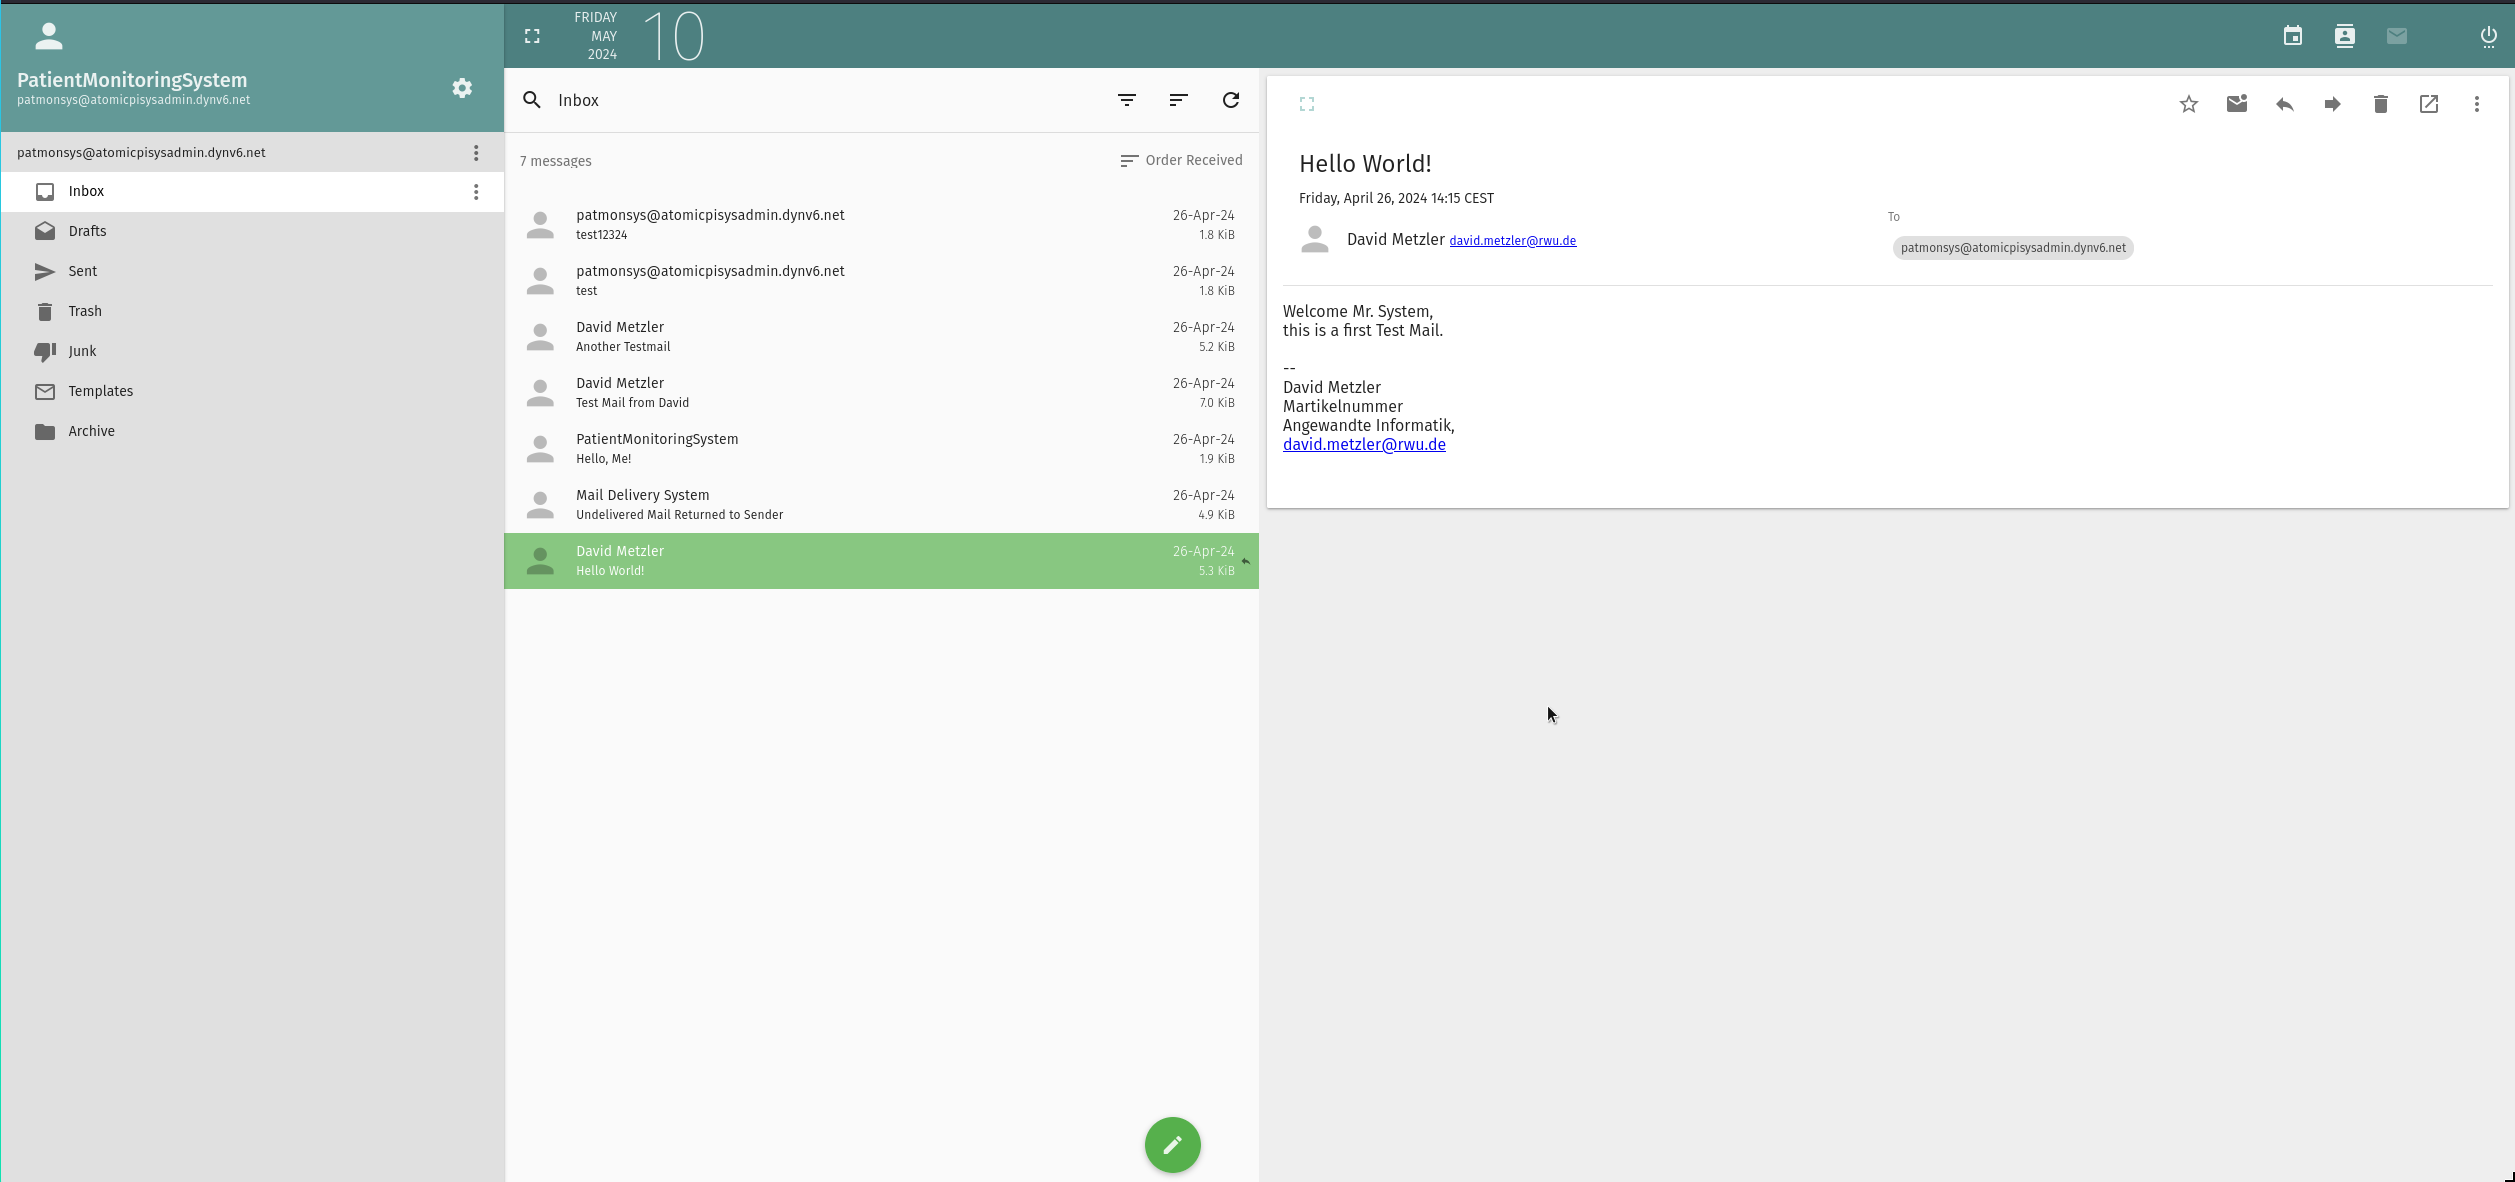
\includegraphics[width=\textwidth]{Images/SGO_Webmail.png}
		\end{minipage}
		\caption{SOGo Weboberfläche für Postfach}
	\end{figure}
\end{frame}

\begin{frame}
	\frametitle{Aktueller Stand}
	\framesubtitle{YOLO}
	
		\begin{enumerate}
		\item Pretrained Model
		\item Container aufgesetzt
		\item Detektion über folgende Klassen:
	\end{enumerate}
	
	\begin{figure}
		\centering
		\begin{minipage}[t]{0.3\textwidth}
			\centering
			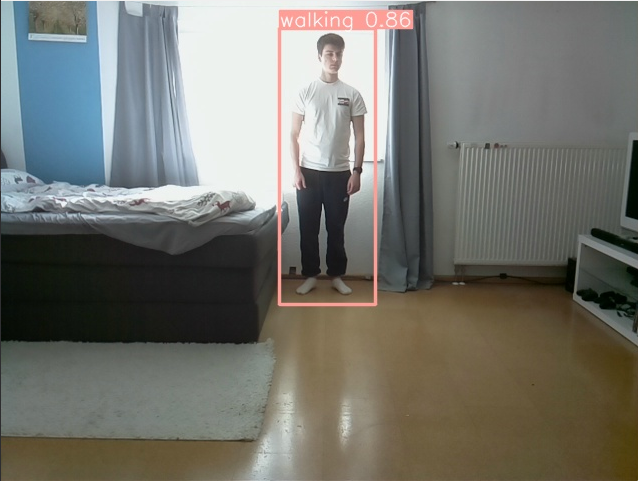
\includegraphics[width=\textwidth]{Images/walking.png}
			\caption*{''walking''}
		\end{minipage}
		\hfill
		\begin{minipage}[t]{0.3\textwidth}
			\centering
			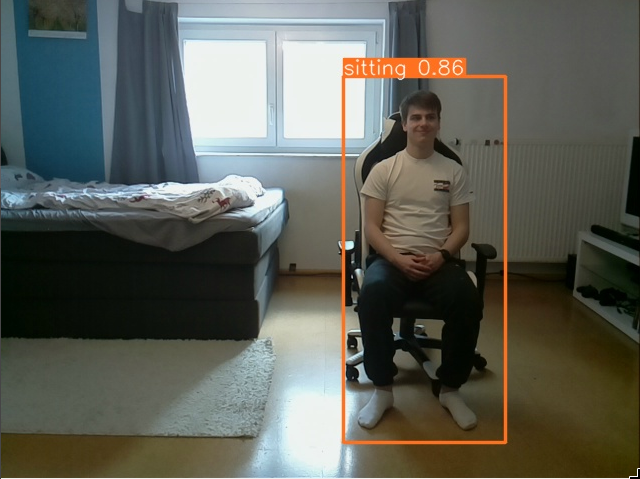
\includegraphics[width=\textwidth]{Images/sitting.png}
			\caption*{''sitting''}
		\end{minipage}
		\hfill
		\begin{minipage}[t]{0.3\textwidth}
			\centering
			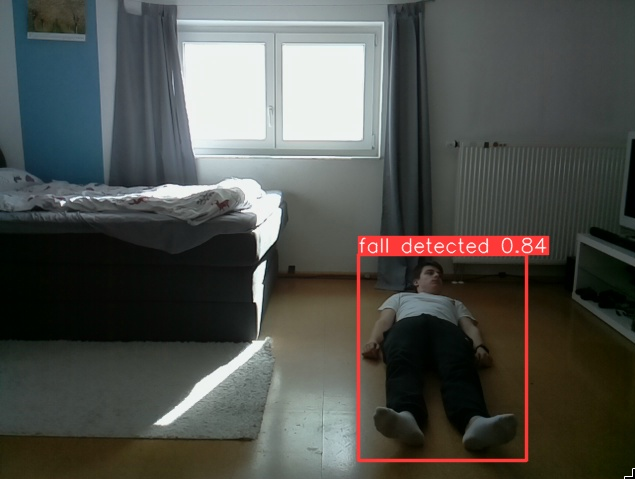
\includegraphics[width=\textwidth]{Images/fallen.png}
			\caption*{ ''fall detected''}
		\end{minipage}
		\caption{YOLOv5 Klassen}
		\label{fig:yolo_classes}
	\end{figure}

\end{frame}



\begin{frame}
	\frametitle{Matrix}	
	\begin{figure}
		\centering
		\begin{tikzpicture}[scale=0.7]
			\node[inner sep=0pt] (laptop1) at (-10,2)
			{
\includegraphics[width=0.15\textwidth]{Images/computer.png}};
			\node[font=\scriptsize] at (-10,1.2) {\scriptsize Laptop 1};
			
			\draw[->] (-9.2,1.8)--(-6.5,0.5) node[pos=0.5, above,rotate=-28] {\scriptsize matrix.org};
			
			\node[inner sep=0pt] (laptop2) at (-10,0)
			{
\includegraphics[width=0.15\textwidth]{Images/computer.png}};
			\node[font=\scriptsize] at (-10,-0.8) {\scriptsize Laptop 2};
			
			\draw[->] (-9,0)--(-6.5,0) node[pos=0.45, above] {\scriptsize matrix.org};
			
			\node[inner sep=0pt] (laptop3) at (-10,-2)
			{
\includegraphics[width=0.15\textwidth]{Images/computer.png}};
			\node[font=\scriptsize] at (-10,-2.8) {\scriptsize Laptop 3};
			
			\draw[->] (-9.2,-1.8)--(-6.5,-0.5) node[pos=0.5, above,rotate=26] {\scriptsize matrix.org};
			
			\node[inner sep=0pt] (internet) at (-5,0)
			{
\includegraphics[width=0.10\textwidth]{Images/cloud.png}};
			\node[font=\scriptsize] at (-5,-0.8) {\scriptsize Internet};
			
			\draw[->] (-4,0)--(-3,0);
			
			\node[inner sep=0pt] (reverseproxy) at (-2,0)
			{
\includegraphics[width=0.10\textwidth]{Images/switch.png}};
			\node[font=\scriptsize] at (-2,-0.7) {\scriptsize reverse proxy};
			
			\draw[->] (-1,0.0)--(0,0);
			
			\node[inner sep=0pt] (matrixserver) at (1,0)
			{
\includegraphics[width=0.10\textwidth]{Images/switch.png}};
			\node[font=\scriptsize] at (1,-0.6) {\scriptsize matrix server};
			
			\draw[<->] (2,0.0)--(3,0);
			
			\node[inner sep=0pt] (datenbank) at (4,0)
			{
\includegraphics[width=0.04\textwidth]{Images/datenbank.png}};
			\node[font=\scriptsize] at (4,-0.6) {\scriptsize PostgresSQL};
			
		\end{tikzpicture}
		\caption{Aufbau des Matrix Servers}
		\label{fig:patient_reverse_proxy}
	\end{figure}
\end{frame}



\begin{frame}
	\frametitle{Matrix Client}
	\begin{figure}
		\centering
		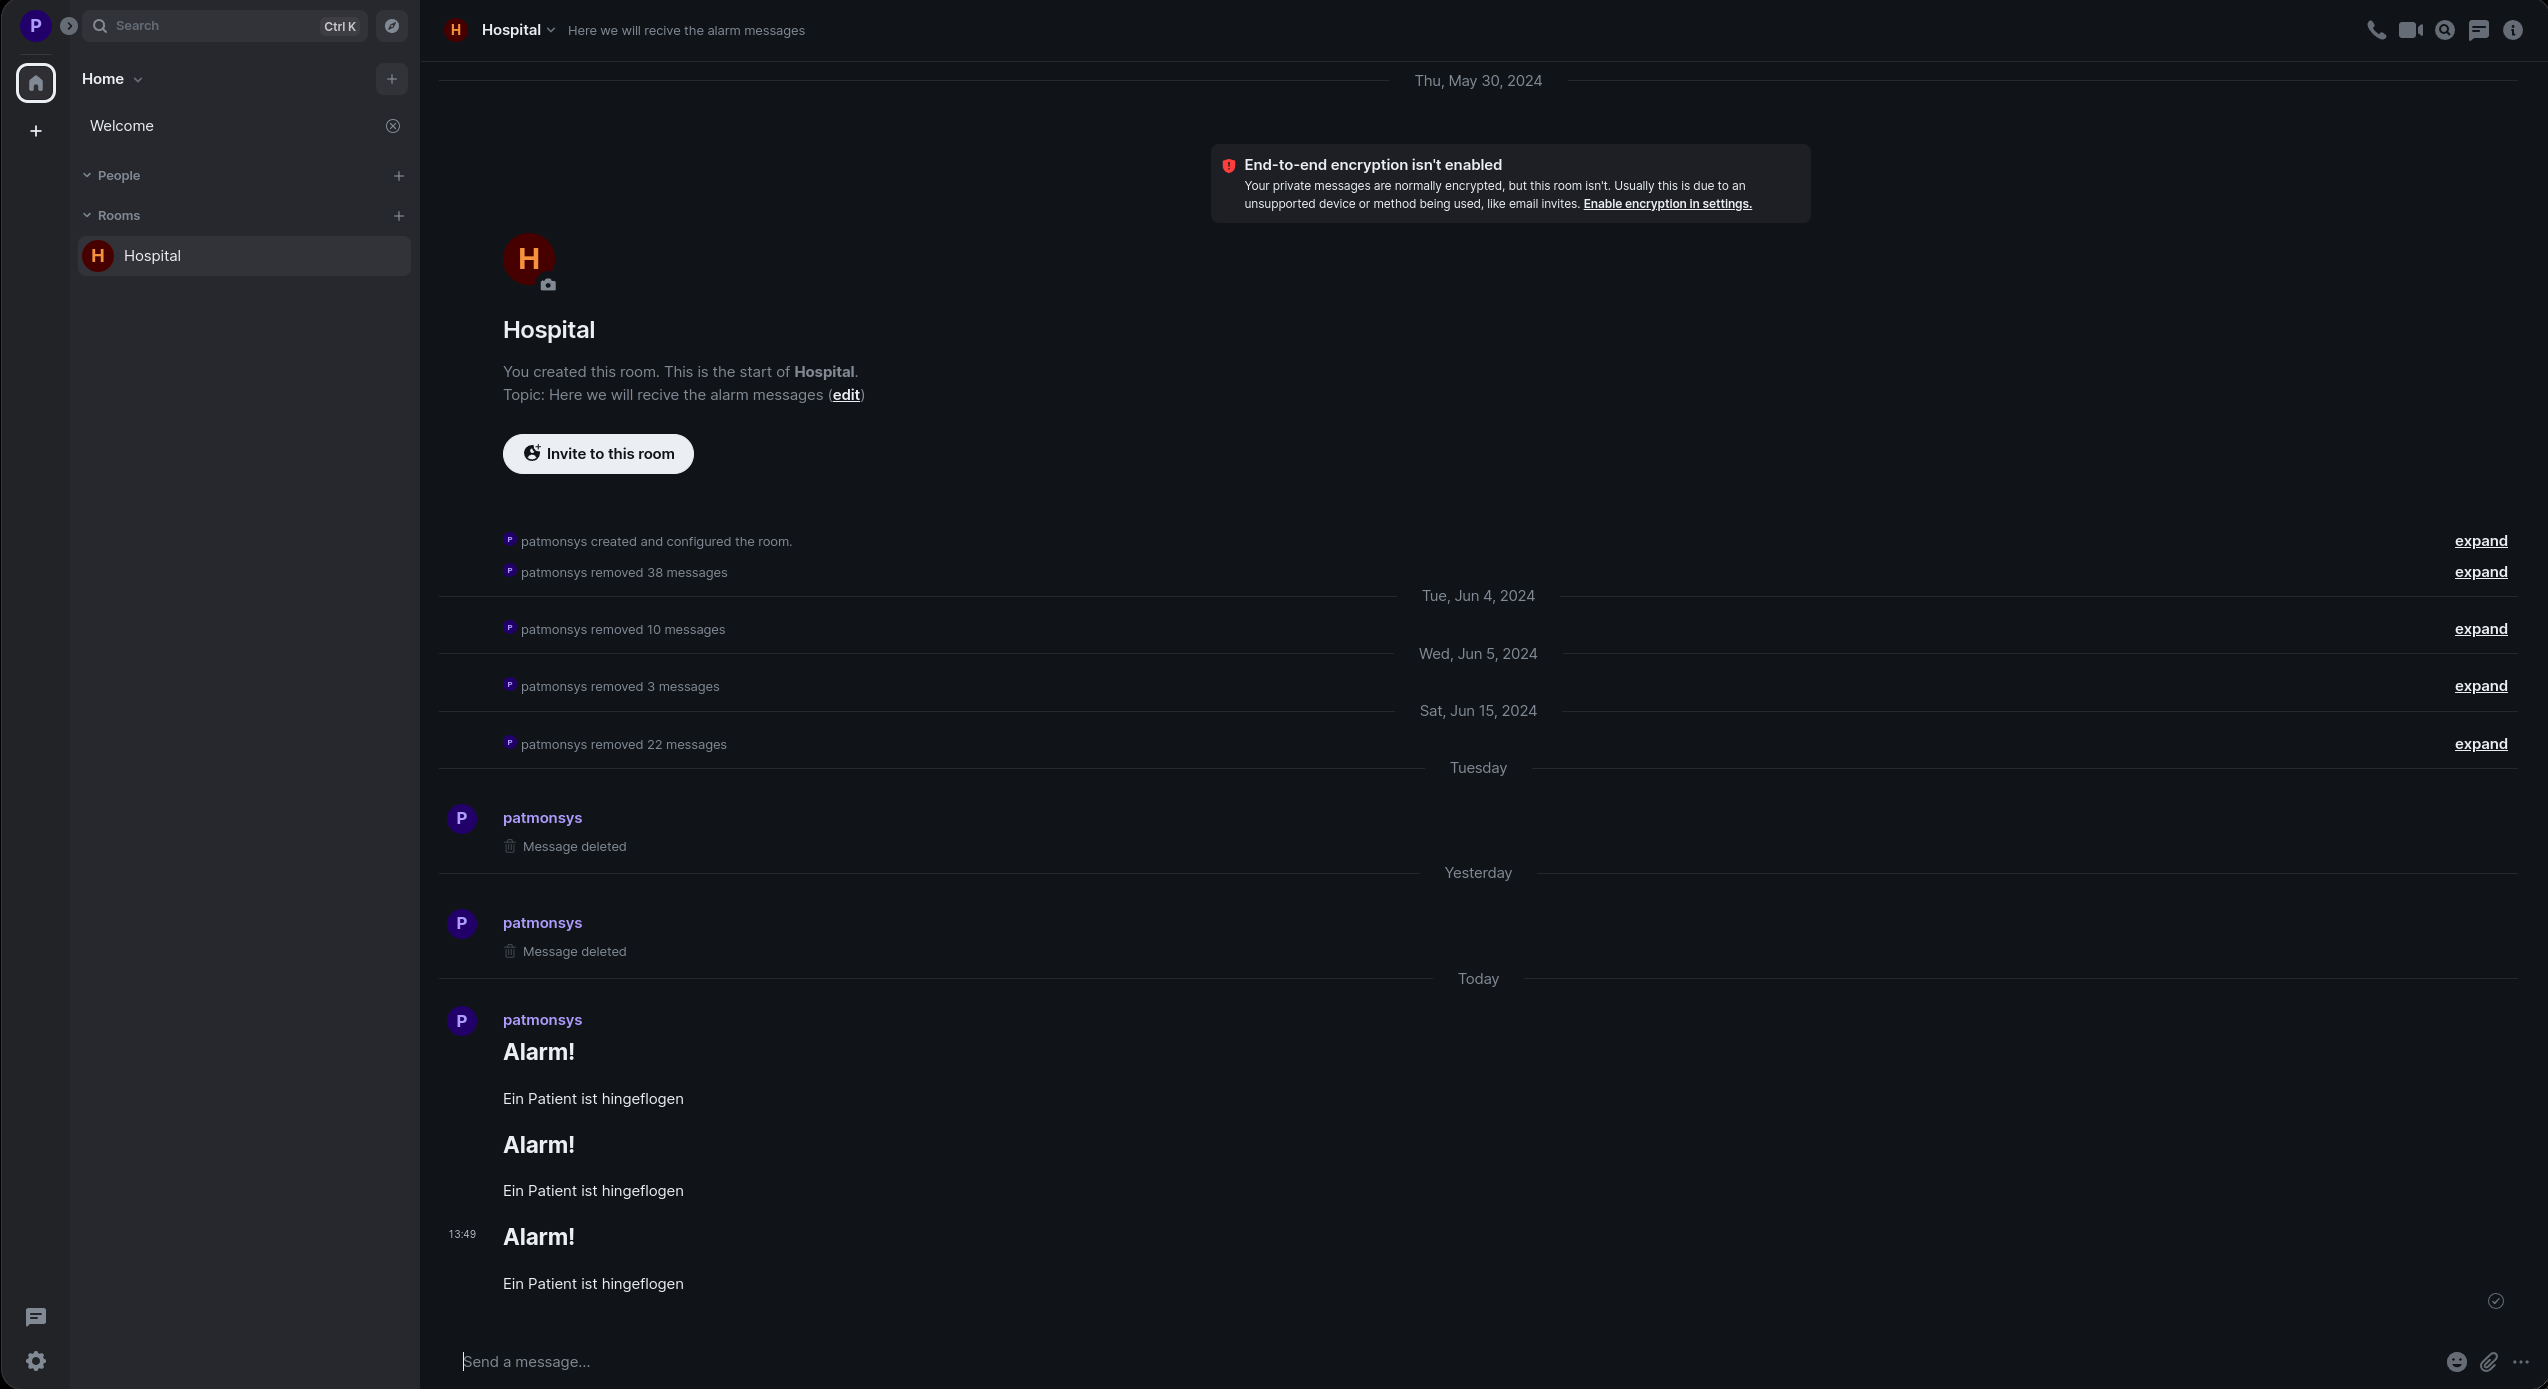
\includegraphics[width=0.8\textwidth]{Images/Matrix.png}
		\caption*{Matrix Room in Element}
		\label{fig:Matrix_Client}
	\end{figure}
\end{frame}



\section{Evauluation}
\begin{frame}
	\frametitle{Evauluation}
	\begin{enumerate}
		\item Zusammenführen der Systeme
		\item Evaluation
		\item Alarm Setup
	\end{enumerate}
\end{frame}

\section{Ausblick}
\begin{frame}
	\frametitle{Ausblick}
	\begin{enumerate}
		\item Bett Detection
		\item Bystander Anonymization
		\item Andere YOLOv8-Modelle 
	\end{enumerate}
\end{frame}

\end{document}
